% !TEX root = quickstep.tex

\section{Scheduling \& Execution} \label{query-exec}
In this section, we describe how the design of the query processing engine in \Quickstep\ achieves three key objectives. First, we believe that separating the control flow and the data flow involved in query processing allows for greater flexibility in reacting to runtime conditions and facilitates maintainability and extensibility of the system. To achieve this objective, the engine separates responsibilities between a scheduler, which makes work scheduling decisions, and workers that execute the data processing kernels (cf. Section~\ref{sec:threading-model}).

Second, to fully utilize the high degree of parallelism offered by modern processors, \Quickstep\ complements its block-based storage design with a work order-based scheduling model (cf. Section~\ref{scheduler}) to obtain high intra-query and intra-operator parallelism.

Finally, to support diverse scheduling policies for sharing resources (such as CPU and memory) between concurrent  queries, the scheduler design separates the choice of policies from the execution mechanisms (cf. Section~\ref{sec:scheduler-policy-vs-mechanism}).

%The scheduler in Quickstep is a crucial component and we describe it in this section. Query execution in \Quickstep\ leverages the block-based storage manager design described in Section~\ref{storage-manager}, and uses a workflow-based query execution paradigm. In \Quickstep, query execution involves generating a series of \textit{work orders} that are then executed by workers. A work order largely corresponds to applying some operation on a block of input tuples (Section~\ref{scheduler} below has more details).

%\subsection{Operator Algorithms} \label{operators}
%In this section, we briefly describe the operator algorithms that are currently implemented in \Quickstep.
%
%\Quickstep\ has a novel implementation of the selection operator where the operator can decide, on a block-by-block basis, what algorithm to use to apply the selection operation. When applying a predicate, the ``micro-optimizer'' (see Section~\ref{vectorization}) may choose to evaluate some or all of the predicate using a fast path like an index lookup
%%(using a BitWeaving or CSB+-Tree index),
%or a binary search on a sorted column in a column-store. If no fast-path is available, the system falls back to iterating over the tuples in a block and evaluating the predicate(s) in a vectorized fashion. The next step in evaluating the selection operation is to materialize the expressions in the projection list (again using vectorized column-at-a-time execution), and bulk-inserting the resultant tuples into a temporary in-memory block for consumption by other operators. In the common case when the projection simply copies column values as is from the input, the expression evaluation component is skipped entirely and data is directly copied from one block into another.
%
%\subsubsection{Hash Join} \label{sec:inline-tuples}
%\Quickstep\ implements a traditional hash join algorithm consisting of a build phase and a probe phase. These phases are implemented as separate operators. The build hash table operator reads blocks of the build relation, and builds a single cache-efficient hash table in memory using the join predicate as the key (borrowing the ideas proposed in~\cite{BlanasLP11}). The probe hash table operator reads blocks of the probe relation, probes the hash table, and materializes joined tuples into in-memory blocks for consumption by other operators, just like the selection operator does. Both the build and probe operators take advantage of block-level parallelism, and use a latch-free concurrent hash table to allow multiple workers to proceed at the same time.
%
%For non-equijoins, \Quickstep\ uses a block-nested loops join algorithm.  %(which also allows a ``residual'' filter predicate to be used with a hash-join to filter joined tuple pairs on a non-equijoin predicate in addition to the equality predicate evaluated by hashing). %Note that the resize operation of hash table is not lock-free.
%
%The basic hash join operator has also been adapted to support left outer join, left semijoin, and antijoin operators.
%
%%An important optimization is used for the hash table, which we describe next.
%
%%\textbf{Inlining tuples in a hash table: } An important issue, which hasn't received much attention in the literature, is how to deal with the payload associated with the entries in a hash table, when used for join evaluation. The common approach is to store in the hash table the key(s) of the build-side tuple along with a pointer/reference to the build tuple. However, this approach may incur a large overhead in retrieving the build tuples when the join is ready to materialize its output and when the result join tuple has build-side attributes that are not part of the join key(s).
%
%%An alternative approach is to store the required build-side attributes (in a row-store format) in the hash table itself. This approach avoids incurring the potentially expensive operation of fetching the build tuple, which is most likely no longer in the processor caches when it is retrieved. (The reason for this behavior is because the task of building the hash table was followed by a batch-based probing of the hash table using the tuples in the current probe block. The probe operation will have likely wiped out the build tuples from the cache.) However, this inlining approach imposes an additional space overhead on the hash table, as the hash table could now be potentially larger. \Quickstep\ uses a simple rule that is based on examining the size of the in-lined tuple and the resulting size of the hash bucket. If this size is smaller than the processor cache line size, then inlining is turned on.
%
%\subsubsection{Aggregation}
%%For aggregation without GROUP BY, the aggregate operator reads blocks of the input relation and generates work orders per block that compute the aggregates local to their assigned block.
%For aggregation without \texttt{GROUP BY}, the operator computes local aggregates for each input block.
%These local aggregates are later merged with the global aggregates for the entire query.
%%For aggregation with GROUP BY, the operator generates work orders per block that together build a (latch-free) hash table of aggregation handles in parallel using the grouping columns as the key.
%For aggregation with \texttt{GROUP BY}, the operator builds a global latch-free hash table of aggregation handles in parallel, using the grouping columns as the key.
%%After processing all the blocks in the input relation, a work order iterates through the hash table to output the grouping keys and their corresponding aggregates, or just the aggregates in the case of aggregation without GROUP BY.
%% Note that this final phaseof iterating through the hash table and output tuples can be parallelized further by
%% assigning parts of the hash table to individual work orders.
%
%\subsubsection{Sort and Top-K}
%\Quickstep\ employs a two-phase algorithm for sorting and top-K operators. These phases are implemented as separate operators. In the first phase, each block of the input relation is sorted in-place, or copied to a single temporary sorted block. This phase is similar to the run generation phase of the traditional external sort. In the second phase, runs of sorted blocks are merged to produce a fully sorted output relation.

\subsection{Threading Model} \label{sec:threading-model}
The \Quickstep\ execution engine consists of a single \textit{scheduler} thread and a pool of \textit{workers}.
The scheduler thread uses the query plan to generate and schedule work for the workers.
When multiple queries are concurrently executing in the system, the scheduler is responsible for enforcing resource allocation policies across concurrent queries and controlling query admittance under high load.
Furthermore, the scheduler monitors query execution progress, enabling status reports as illustrated in Section~\ref{sec:progress-monitoring}.

The workers are responsible for executing the relational operation tasks that are scheduled.
Each worker is a single thread that is pinned to a CPU core (possibly a virtual core), and there are as many workers as cores available to \Quickstep.
The workers are created when the Quickstep process starts, and are kept alive across query executions, minimizing query initialization costs.
The workers are stateless; thus, the worker pool can \textit{elastically} grow or shrink dynamically. %at any time in the database process' runtime.
%It is possible to \textit{elastically} add new workers to the pool while a query is under execution, to provide more parallelism.
%Workers are always stateless, so the scheduler can terminate them either at process termination, after all queries have been completed or cancelled, or even mid-query, in order to react to changes in resource availability.
%This property of ``elasticity'' is illustrated in Section~\ref{sec:expt:elasticity}.
% The elasticity comment is a left over from the previous versions of this paper.
%\reminder{I'm not sure what poison work orders do. Do they terminate the threads? If so, why would we do that to abort a query?}

%The unit of work scheduled by the scheduler is called a \textit{work order}, and is described in the next section.

%The \Quickstep\ execution engine uses two kinds of execution threads, namely \textit{foreman} and \textit{worker} threads.
%
%\textit{Worker threads} execute work orders produced by physical relational operators. The \textit{foreman thread} makes decisions about scheduling the work orders to the Worker threads.
%%The current execution engine allows a single query to be controlled by a single foreman thread.
%All worker threads are stateless. They simply keep executing work orders in a loop. A worker thread can be terminated by sending a special \textit{poison work order}. The work order termination method can then be used to gracefully terminate the \Quickstep\ process, or to abort a query (for example, in response to the client issuing a query cancellation command). %Concurrent queries are supported, and a foreman thread is spawned for every new query that arrives into the system.
%
%To minimize the thread initialization costs, all the Worker threads are created when the \Quickstep\ process is started, and they stay alive until the \Quickstep\ process terminates.
%However, since workers are stateless, it is easy to add or remove them, even mid-query.
%
%All worker threads can be pinned to CPU cores to avoid migration costs when the operating system (OS) decides to move a thread from one CPU core to another.

\subsection{Work Order-based Scheduler}\label{scheduler}
The \Quickstep\ scheduler divides the work for the entire query into a series of \textit{work orders}. In this section,
%we describe this work order-based scheduler.
we first describe the work order abstraction and provide a few example work order types. Next, we explain how the scheduler generates work orders for different relational operators in a query plan, including handling of pipelining and internal memory management during query execution.
%We also explain how the \Quickstep\ scheduler handles query execution aspects such as pipelining and internal memory management during a query execution.

\begin{figure}
\centering
   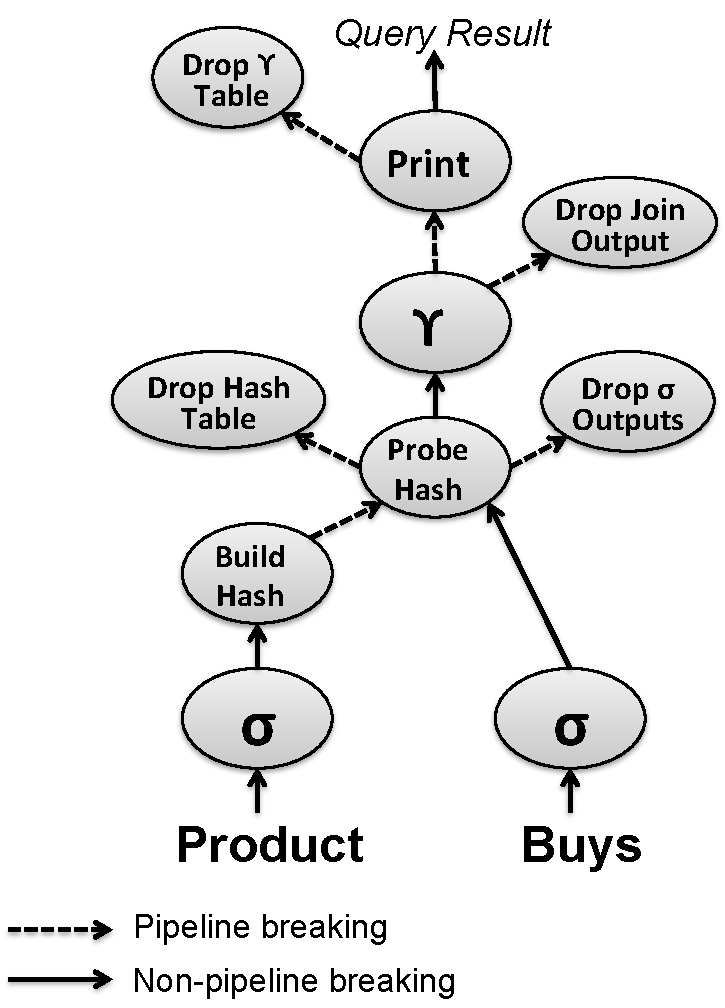
\includegraphics[width=.35\textheight]{system/figures/physical-plan.pdf}
   \caption{\textbf{Plan DAG for the sample query}}
   \label{fig-dag}
\end{figure}

The optimizer sends to the scheduler an execution query plan represented as a directed acyclic graph (DAG) in which each node is a relational operator. Figure~\ref{fig-dag} shows the DAG for the example query shown below. Note that the edges in the DAG are annotated with whether the producer operator is blocking or permits pipelining.
%consumer operator is blocked on the output produced by the producer operator, or whether data pipelining is allowed between neighboring operators.

%The optimal query plan that is produced by the optimizer is converted to a DAG of operators.
%This DAG representation of the query is then sent to the scheduler.

\begin{lstlisting}[language=SQL,upquote=true,
basicstyle=\ttfamily\small,
showstringspaces=false,
keywordstyle=\color{cardinal}\bfseries,
emphstyle=\color{bondiblue}\bfseries,
stringstyle=\color{bondiblue}\bfseries,
emph={SUM}]
  SELECT SUM(sales)
  FROM   Product P NATURAL JOIN Buys B
  WHERE  B.buy_month = 'March'
  AND    P.category = 'swim'
\end{lstlisting}

\subsubsection{Work Order}

%Each relational operator presents the work that needs to be done to execute the query using \textit{work orders}.
A \textit{work order} is a unit of intra-operator parallelism for a relational operator. Each relational operator in Quickstep describes its work in the form of a set of work orders, which contains references to its inputs and all its parameters.
%For concreteness, we describe some sample work orders for few relational operators.
For example, a \textit{selection work order} contains a reference to its input relation, a filtering predicate, and a projection list of attributes (or expressions) as well as a reference to a particular input block. A selection operator generates as many work orders as there are blocks in the input relation. Similarly, a \textit{build hash work order} contains a reference to its input relation, the build key attribute, a hash table reference, and a reference to a single block of the input build relation to insert into the hash table.

\subsubsection{Work Order Generation and Execution}
%We now describe the work orders generation for a given query plan.

The scheduler employs a simple DAG traversal algorithm to activate nodes in the DAG.
An active node in the DAG can generate \textit{schedulable} work orders, which can be fetched by the scheduler.
In the example query, initially, only the Select operators (shown in Figure~\ref{fig-dag} using the symbol $\sigma$) are active. Operators such as the probe hash and the aggregation operations are initially inactive as their blocking dependencies have not finished execution.
The scheduler begins executing this query by fetching work orders for the select operators. Later, other operators will become active as their dependencies are met, and the  scheduler will fetch work orders from them.
% and they generate work orders -- one for each input block from both input relations.

The scheduler assigns these work orders to available workers, which then execute them. All output is written to temporary storage blocks. After executing a work order, the worker sends a completion message to the scheduler, which includes execution statistics that can be used %by the scheduler
to analyze the query execution behavior.

\subsubsection{Implementation of Pipelining}
In our example DAG (Figure~\ref{fig-dag}), the edge from the Probe hash operator to the Aggregate operator allows for data pipelining.
As described earlier, the output of each probe hash work order is written in some temporary blocks.
Fully-filled output blocks of probe hash operators can be streamed to the aggregation operator (shown using the symbol $\gamma$ in the figure).
The aggregation operator can generate one work order for each streamed input block that it receives from the probe operator, thereby achieving pipelining.

The design of the Quickstep scheduler separates control flow from data flow.
The control flow decisions are encapsulated in the work order scheduling policy.
This policy can be tuned to achieve different objectives, such as aiming for high performance, staying with a certain level of concurrency/CPU resource consumption for a query, etc.
In the current implementation, the scheduler \textit{eagerly} schedules work orders as soon as they are available.

\subsubsection{Output Management}
During query execution, intermediate results are written to temporary blocks. To minimize internal fragmentation and amortize block allocation overhead, workers reuse blocks belonging to the same output relation until they become full. To avoid memory pressure, these intermediate relations are dropped as soon as they have been completely consumed (see the Drop $\sigma$ Outputs operator in the DAG). Hash tables are also freed similarly (see the Drop Hash Table operator). An interesting avenue for future work is to explore whether delaying these Drop operators can allow sub-query reuse across queries.

 \subsection{Separation of Policy and Mechanism} \label{sec:scheduler-policy-vs-mechanism}

Quickstep's scheduler supports concurrent query execution. Recall that a query is decomposed into several work orders during execution. These work orders are organized in a data structure called the \textit{Work Order Container}. The scheduler maintains one such container per query. A \textit{single scheduling decision} involves: selection of a query $\rightarrow$ selection of a work order from the container $\rightarrow$ dispatching the work order to a worker thread. When concurrent queries are present, a key aspect of the scheduling decision is to select a query from the set of active concurrent queries, which we describe next.

The selection of a query is driven by a \textit{high level policy}. An example of such a policy is \textit{Fair}. With this policy, in a given time interval, all active queries get an equal proportion of the total CPU cycles across all the cores. Another such policy is \textit{Highest Priority First} (HPF), which gives preference to higher priority queries. (The HPF policy is illustrated later in Section~\ref{sec:expt:elasticity}.) Thus, \Quickstep's scheduler consists of a component called the \textit{Policy Enforcer} that transforms the policy specifications in each of the scheduling decisions.

The Policy Enforcer uses a \textit{probabilistic framework} for selecting queries for scheduling decisions. It assigns each query a probability value, which indicates the likelihood of that query being selected in the next scheduling decision. %Thus, each scheduling decision is probabilistic and uses the probability value assigned to each query.
We employ a probabilistic approach because it is attractive from an implementation and debugging perspective (as we only worry about the probability values, which can be adjusted dynamically at anytime, including mid-way through query execution).

The probabilistic framework forms the \textit{mechanism} to realize the high level policies and remains decoupled from the policies.
This design is inspired from the classical \textit{separation of policies from mechanism} principle~\cite{LampsonS76}.

A key challenge in implementing the Policy Enforcer lies in transforming the policy specifications to probability values, one for each query.
A critical piece of information used to determine the probability values is the prediction of the execution time of the future work order for a query.
This information provides the Policy Enforcer some insight into the future resource requirements of the queries in the system.
The Policy Enforcer is aware of the current resource allocation to different queries in the system, and using these predictions, it can adjust the future resource allocation with the goal of \textit{enforcing} the specified policy for resource sharing.

The predictions about execution time of future work orders of a query are provided by a component called the \textit{Learning Agent}.
It uses a prediction model that takes execution statistics of the past work orders of a query as input and estimates the execution time for the future work orders for the query.

The calculation of the probability values for different policies implemented in \Quickstep\, and their relation with the estimated work order execution time is presented in~\cite{DBLP:conf/bigdata/DeshmukhMP17}.

To prevent the system from thrashing (e.g. out of memory), a load controller is in-built into the scheduler.
During concurrent execution of the queries, the load controller can control the admission of queries into the system and it may suspend resource intensive queries, to ensure resource availability.

\begin{figure*}[t]
\centering
\begin{subfigure}[bt]{0.3\textwidth}
  \centering
   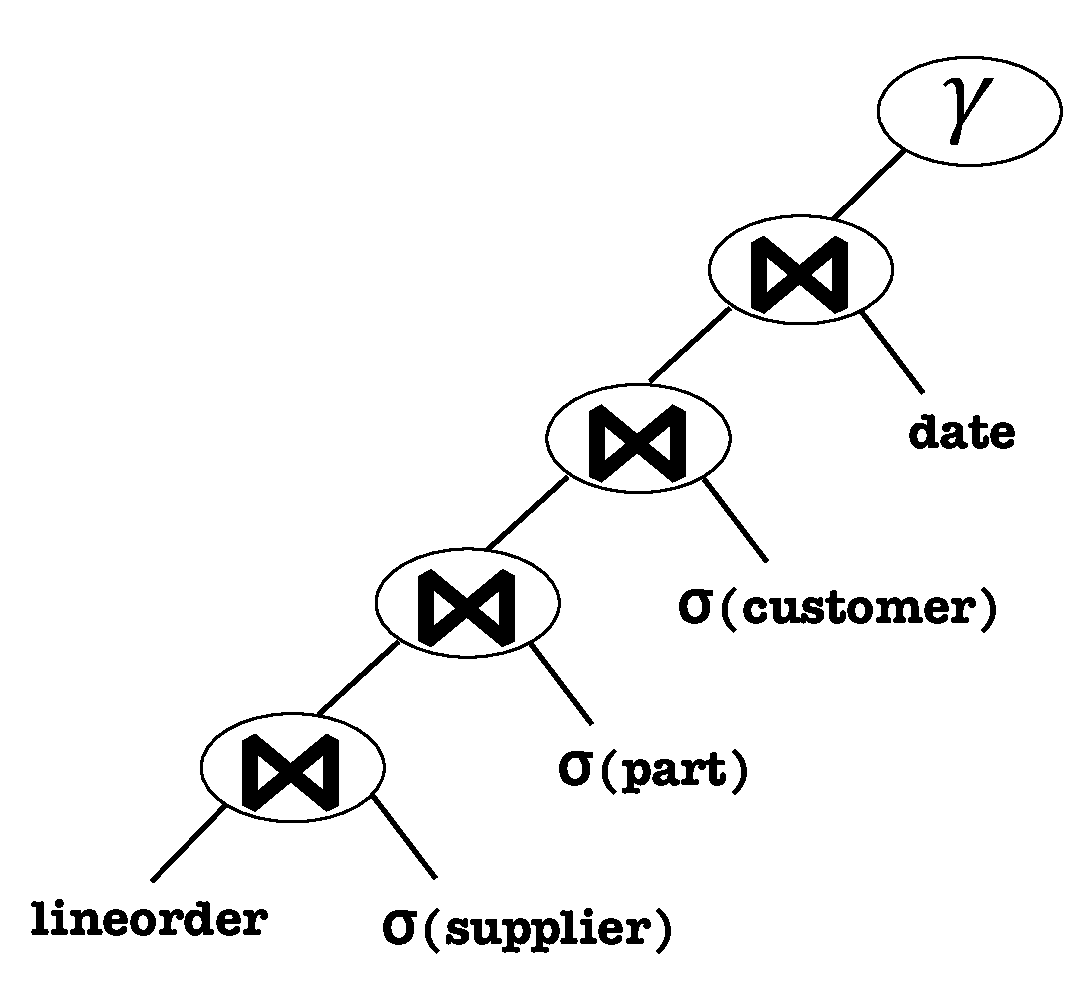
\includegraphics[width=1.0\textwidth,
                    height=0.75\textwidth]{system/figures/Q41-original.pdf}
   \caption{Original query plan}
   \label{fig-q41-original}
\end{subfigure} %
\begin{subfigure}[bt]{0.3\textwidth}
  \centering
   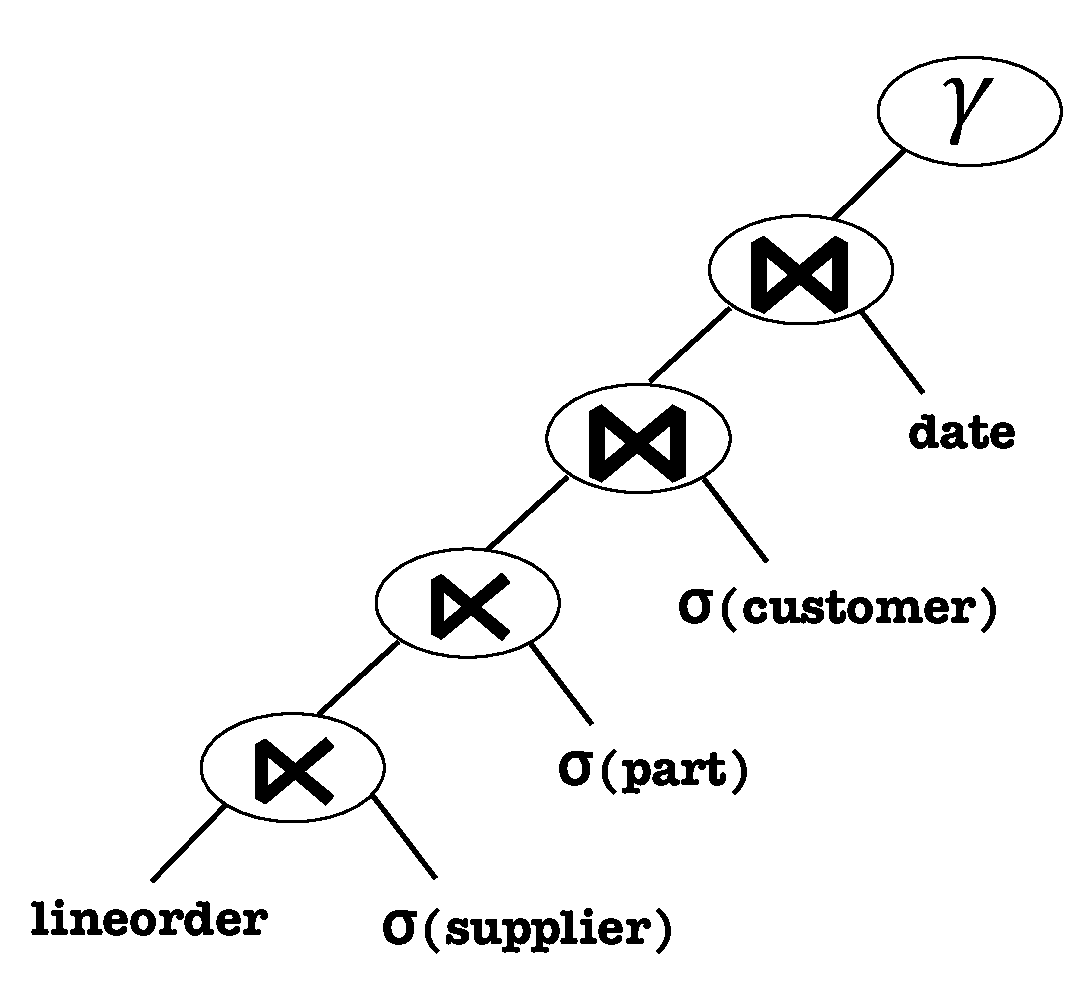
\includegraphics[width=1.0\textwidth,
                    height=0.75\textwidth]{system/figures/Q41-semijoin.pdf}
   \caption{Plan using join to semi-join transformation}
   \label{fig-q41-semijoin}
\end{subfigure} %
\begin{subfigure}[bt]{0.3\textwidth}
  \centering
   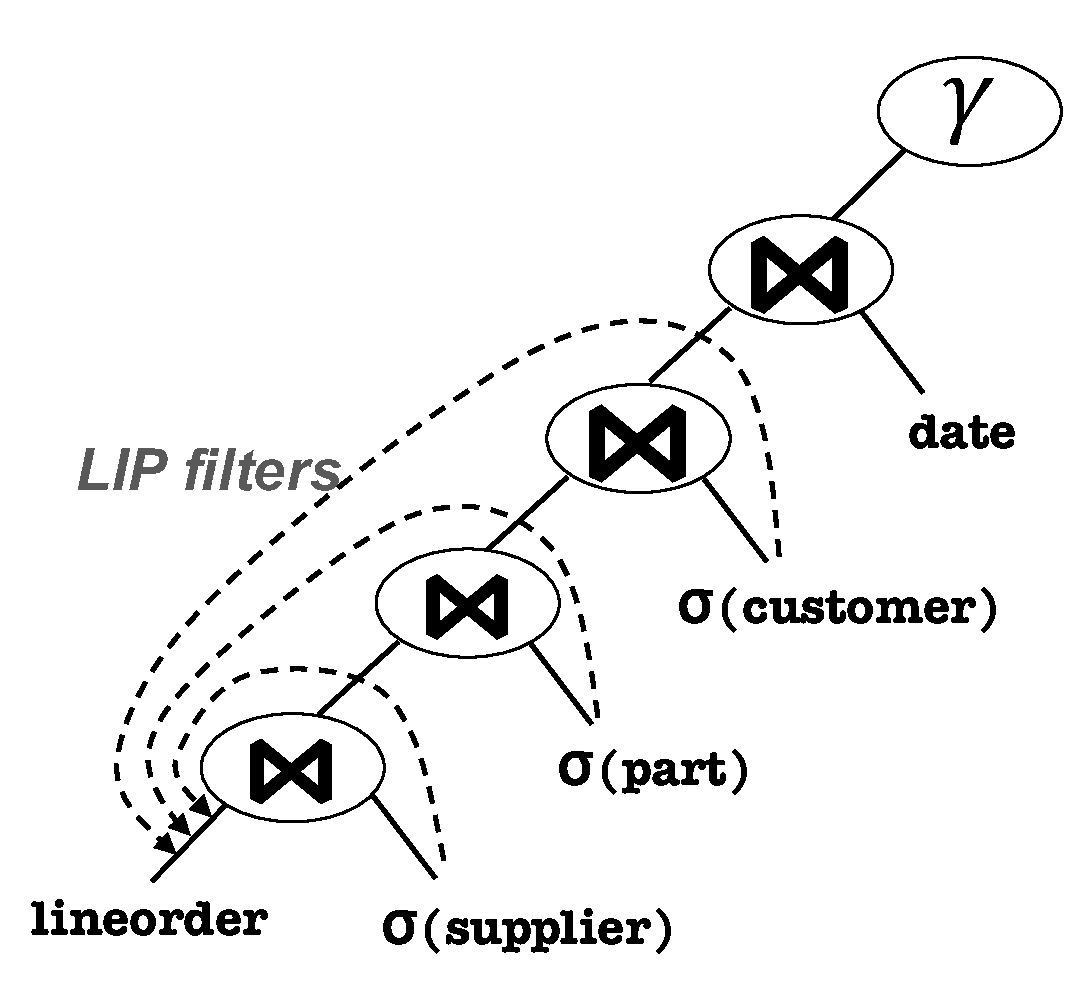
\includegraphics[width=1.0\textwidth,
                    height=0.75\textwidth]{system/figures/Q41-LIP.pdf}
   \caption{Query plan using LIP (only)}
   \label{fig-q41-lip}
\end{subfigure} %
\caption{\textbf{Query plan variations for SSB Query 4.1}}
\end{figure*}

Finally, we note that by simply tracking the work orders that are completed, Quickstep can provide a built-in generic query progress monitor (shown in Section~\ref{sec:progress-monitoring}).
